\documentclass[a4paper]{article}

% Set for specific document
\def\DOCTITLE{CSC3621 Coursework 1 Exercise 2}
\def\DOCAUTHOR{Dan Nixon (120263697)}
\def\DOCDATE{16/10/2015}

% Set document attributes
\title{\DOCTITLE}
\author{\DOCAUTHOR}
\date{\DOCDATE}

\usepackage{fullpage}
\usepackage{scrextend}
\usepackage{titlesec}
\usepackage{fancyhdr}
\usepackage{hyperref}
\usepackage[section]{placeins}
\usepackage{minted}
\usepackage{booktabs}

% Handle graphics correctly
\ifx\pdftexversion\undefined
\usepackage{graphicx}
% \usepackage[dvips]{graphicx}
\else
\usepackage[pdftex]{graphicx}
\DeclareGraphicsRule{*}{mps}{*}{}
\fi

% Setup headers and footers
\pagestyle{fancy}
\lhead{}
\chead{\DOCTITLE}
\rhead{}
\rfoot{\DOCDATE}
\cfoot{\thepage}
\lfoot{\DOCAUTHOR}

% Set header and footer sizes
\renewcommand{\headrulewidth}{0.4pt}
\renewcommand{\footrulewidth}{0.4pt}
\setlength{\headheight}{15.2pt}
\setlength{\headsep}{15.2pt}

% For the sake of not having to repeat the accent escape
\newcommand{\Vigenere}{Vigen\`{e}re }

\begin{document}

\section{\Vigenere cipher program}
\label{sec:vigenere_program}

The \Vigenere encryption and decryption program is implemented in the
\texttt{Vigenere} Java class and executed using the command line interface
implemented in the \texttt{VigenereApp.java} file.

The \texttt{ex2\_run\_cipher\_decipher\_cycle} Bash script demonstrates using
the program to encrypt the \texttt{pg1661.txt} file using the key \textit{ncl}
and then decrypt the text just encrypted.

The \texttt{ex2\_encrypt\_newcastleuniversity} shows the results of encrypting
the text \textit{newcastleuniversity} with key \textit{ncl}, the results of this
are shown in figure \ref{fig:encrypt_newcastleuniversity_result}. This gave the
cipher text \textit{aghpcdgnphptigcfkel}.

\begin{figure}[h!]
  \centering
  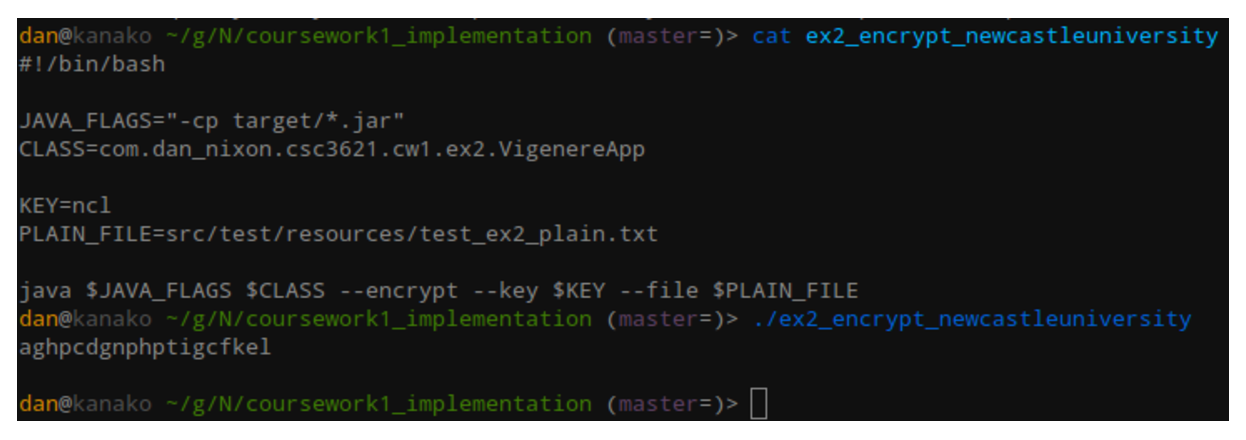
\includegraphics[width=0.8\textwidth]{graphics/ex2_encrypt_newcastleuniversity_result.eps}
  \caption{Encryption of the message \textit{newcastleuniversity}}
  \label{fig:encrypt_newcastleuniversity_result}
\end{figure}

The logic of the program is to iterate through all characters in the plain text
and assuming the character is an English alphabetical character the character is
shifted according to the current position in the key, the key position is
advanced with every character that is rotated until the end of the key is
reached at which point the key position is reset to the start of the key.

\section{Comparison of letter frequencies}

The \texttt{ex2\_compare\_ciphertext\_frequencies} Bash script is used to
perform frequency analysis on a sample of plain English text (in this case the
\texttt{pg1661.txt} file), text encrypted with a simple shift cipher (the
\texttt{Exercise1Ciphertext.txt} file) and a text encrypted with the \Vigenere
cipher (the decrypted plain text from exercise 1 encrypted with the \Vigenere
cipher using the hey \textit{ncl}).

This analysis was performed using the frequency analysis tool developed as part
of exercise 1.

The results of this analysis are shown in table
\ref{table:letter_frequency_comparison}.

\begin{table}[h]
  \centering
  \begin{tabular}{@{}lrrr@{}}
    \toprule
    Letter & Plain English Text & Shift Cipher & \Vigenere cipher \\
    \midrule
    a      & 8.082\%            & 2.657\%      & 3.986\%          \\
    b      & 1.484\%            & 0.265\%      & 2.392\%          \\
    c      & 2.483\%            & 1.661\%      & 4.717\%          \\
    d      & 4.271\%            & 0.0\%        & 3.056\%          \\
    e      & 12.287\%           & 7.774\%      & 5.780\%          \\
    f      & 2.093\%            & 1.395\%      & 4.916\%          \\
    g      & 1.855\%            & 2.923\%      & 6.843\%          \\
    h      & 6.615\%            & 3.654\%      & 2.657\%          \\
    i      & 6.988\%            & 13.621\%     & 1.262\%          \\
    j      & 0.121\%            & 1.594\%      & 3.122\%          \\
    k      & 0.823\%            & 2.126\%      & 1.461\%          \\
    l      & 3.944\%            & 5.714\%      & 3.787\%          \\
    m      & 2.718\%            & 7.242\%      & 0.598\%          \\
    n      & 6.649\%            & 0.199\%      & 5.182\%          \\
    o      & 7.798\%            & 0.598\%      & 3.122\%          \\
    p      & 1.629\%            & 3.720\%      & 7.308\%          \\
    q      & 0.097\%            & 2.857\%      & 3.787\%          \\
    r      & 5.743\%            & 6.843\%      & 6.843\%          \\
    s      & 6.254\%            & 6.578\%      & 2.192\%          \\
    t      & 9.059\%            & 2.392\%      & 5.847\%          \\
    u      & 3.049\%            & 0.265\%      & 4.518\%          \\
    v      & 1.022\%            & 6.710\%      & 6.112\%          \\
    w      & 2.574\%            & 7.508\%      & 2.325\%          \\
    x      & 0.129\%            & 7.973\%      & 1.196\%          \\
    y      & 2.182\%            & 2.923\%      & 3.853\%          \\
    z      & 0.034\%            & 0.797\%      & 3.122\%          \\
    \bottomrule
  \end{tabular}
  \caption{Letter frequencies in shift and \Vigenere ciphers}
  \label{table:letter_frequency_comparison}
\end{table}

This shows that although the \Vigenere cipher does produce cipher text that has
a more even probability distribution than a shift cipher, it still contains a
pattern which can be exploited as demonstrated in section
\ref{sec:cryptanalysis}.

\section{Cryptanalysis of \Vigenere cipher text}
\label{sec:cryptanalysis}

Retrieving the original message from the cipher text is done in in stages;
discovering the length of the key, for each character of the key obtaining its
value and decrypting the cipher text using the discovered key.

\subsection{Obtaining the key length}

One method of obtaining the length of the key used to encrypt the cipher text
is to examine the index of coincidence of the cipher text.

The index of coincidence is calculated in the \texttt{IOCAnalysis} class using
equation \ref{eq:ioc}, this can then be used to determine a likely key size used
in the encryption and is implemented in the \texttt{obtainKeySize()} method, in
this case the mapping of index of coincidence to key size is enumerated in the
\texttt{keySizeFromIoC()} method.

\begin{equation}
  IC = \frac{\sum_{i = 0}^{25} c_{i} \left(c_{i} - 1\right)}{N \left(N - 1\right)}
  \label{eq:ioc}
\end{equation}
\FloatBarrier

where $c$ is the number of counts for a letter in the text and $N$ is the total
number of letters in the text.

When used on the provided cipher text (\texttt{Exercise2Ciphertext.txt}) this
analysis method gave the most likely key to be 3, however when I attempted to
obtain the key characters using this key length I was unable to successfully
determine a shift offset for the three key positions.

In order to validate that a key length was possible on a given cipher text I
implemented a test in the \texttt{validateKeySize()} function which will split
the cipher text into a given number of columns based on the key size to be
tested and calculate the index of coincidence of each column, if the key is
correct then the index of coincidence will be close to that of plain English
text for every column.

As expected the key size of 3 did not pass this validation test, I therefore
wrote another function, \texttt{obtainKeySizeBruteForce()}, which would iterate
over a given range of key sizes and return the first key size to pass the
\texttt{validateKeySize()} test.

This brute force method returned a key size of 5, which in the next section will
prove to be the correct key length for this cipher text.

\subsection{Obtaining the key characters}

Given the key length, the key characters can be obtained by tabulating the
cipher text into $n$ columns, where $n$ is the size of the key. Then the
frequency analysis described in exercise 1 can be applied to each column
individually to obtain the offset of the shift cipher that encrypted every
character in that column.

In the cryptanalysis program this is implemented in the
\texttt{VigenereAnalysis} Java class, specifically in the
\texttt{frequencyAnalysis()} and \texttt{obtainKey()} methods.

In the case of the provided cipher text this analysis successfully obtains all
five characters of the key (shown in sections \ref{sec:cryptanalysis_output} and
\ref{sec:plaintext}): \textit{plato}.

\subsection{Output of the cryptanalysis program}
\label{sec:cryptanalysis_output}

Figure \ref{fig:cryptanalysis_output} shows the output from the cryptanalysis
program when executed using the \texttt{ex2\_ciphertext\_analysis} Bash script.

Note that the \texttt{--verbose} option is commented out here, if this option is
provided then the probability distributions are output for each letter of the
key to assist in manual analysis if required.

\begin{figure}[h!]
  \centering
  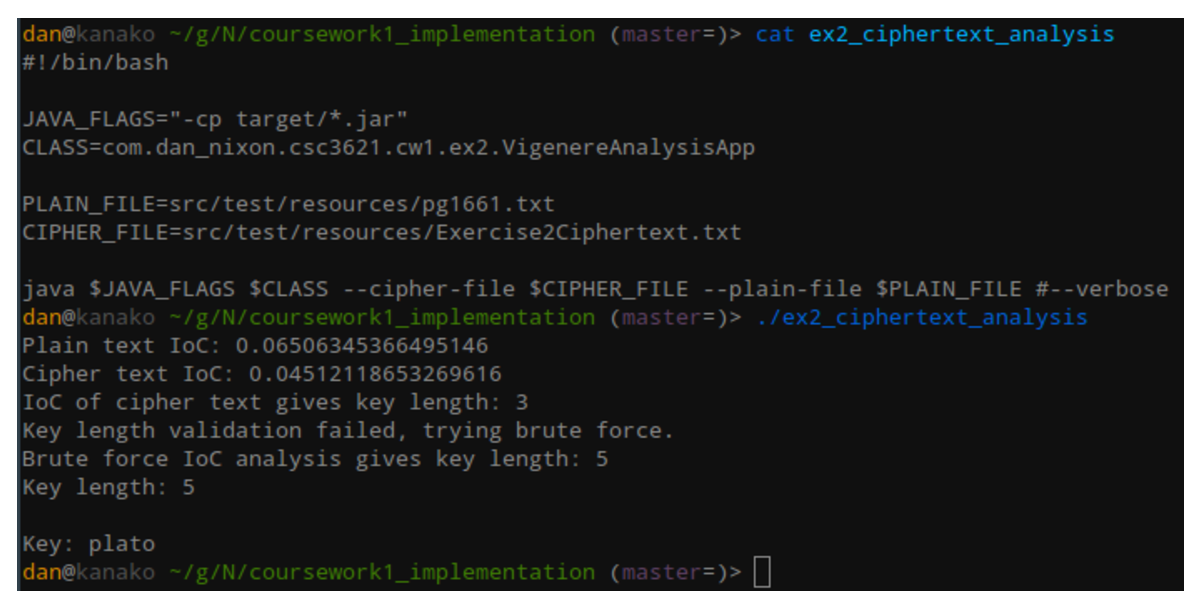
\includegraphics[width=0.8\textwidth]{graphics/ex2_cryptanalysis_output.eps}
  \caption{Output of cryptanalysis program}
  \label{fig:cryptanalysis_output}
\end{figure}

This shows that the program first tries to obtain the key size through the index
of coincidence of the entire cipher text but fails the verification step, then
successfully obtains it through the brute force method.

\subsection{Obtaining the original plain text}
\label{sec:plaintext}

This was done using the program described in section \ref{sec:vigenere_program}
using the \texttt{ex2\_decipher\_set\_ciphertext} Bash script. This gives the
output seen in figure \ref{fig:plaintext_output} (note that the output shown
is truncated in order to save space, however the recurrence of the key several
times).

\begin{figure}[h!]
  \centering
  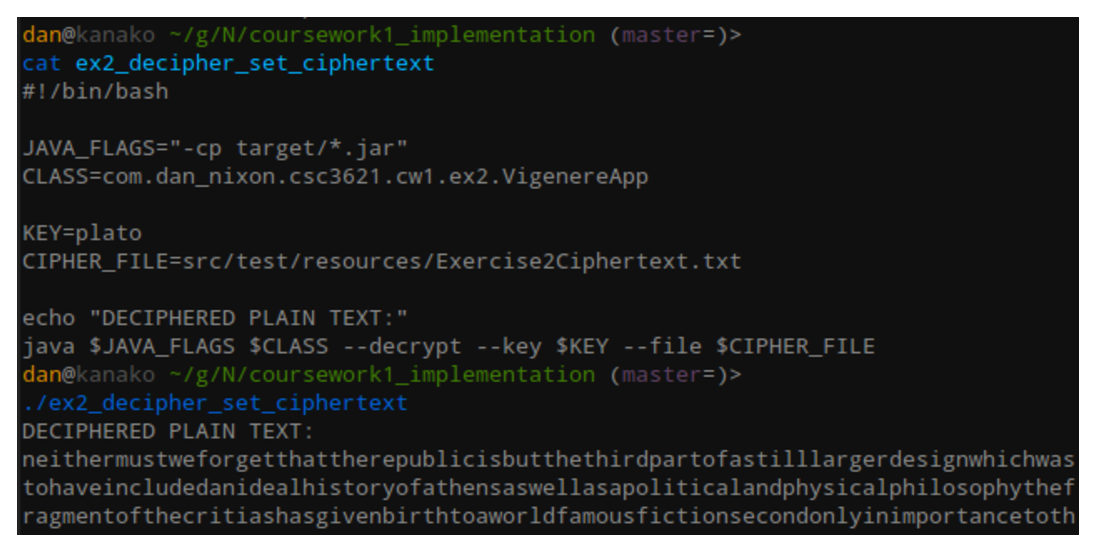
\includegraphics[width=0.8\textwidth]{graphics/ex2_plaintext_output.eps}
  \caption{Decryption of cipher text}
  \label{fig:plaintext_output}
\end{figure}

This clearly shows a comprehensible English sentence; \textit{Neither must we
forget thet there public is but the third part of a still larger design \ldots}.

\end{document}
